% $Header: /cvsroot/latex-beamer/latex-beamer/examples/beamerexample5.tex,v 1.22 2004/10/08 14:02:33 tantau Exp $

\documentclass[11pt]{beamer}
\date{\today}

\usetheme{Darmstadt}

\usepackage{times}
\usefonttheme{structurebold}

%\usepackage[english]{babel}
\usepackage[brazilian]{babel}
\usepackage{pgf,pgfarrows,pgfnodes,pgfautomata,pgfheaps}
\usepackage{amsmath,amssymb}
\usepackage[utf8]{inputenc}
\usepackage{graphicx}

\setbeamercovered{dynamic}

\newcommand{\Lang}[1]{\operatorname{\text{\textsc{#1}}}}

\newcommand{\Class}[1]{\operatorname{\mathchoice
  {\text{\sf \small #1}}
  {\text{\sf \small #1}}
  {\text{\sf #1}}
  {\text{\sf #1}}}}

\newcommand{\NumSAT}      {\text{\small\#SAT}}
\newcommand{\NumA}        {\#_{\!A}}

\newcommand{\barA}        {\,\bar{\!A}}

\newcommand{\Nat}{\mathbb{N}}
\newcommand{\Set}[1]{\{#1\}}

\pgfdeclaremask{tu}{beamer-tu-logo-mask}
\pgfdeclaremask{computer}{beamer-computer-mask}
\pgfdeclareimage[interpolate=true,mask=computer,height=2cm]{computerimage}{beamer-computer}
\pgfdeclareimage[interpolate=true,mask=computer,height=2cm]{computerworkingimage}{beamer-computerred}
\pgfdeclareimage[mask=tu,height=.5cm]{logo}{logounesp}

\logo{\pgfuseimage{logo}}

\title{Entropia e Distribuição de Boltzmann}
\author{Ney Lemke}
\institute[IBB-UNESP]{%
    Departamento de Biofísica e Farmacologia}
\date{\today}                                

\colorlet{redshaded}{red!25!bg}
\colorlet{shaded}{black!25!bg}
\colorlet{shadedshaded}{black!10!bg}
\colorlet{blackshaded}{black!40!bg}

\colorlet{darkred}{red!80!black}
\colorlet{darkblue}{blue!80!black}
\colorlet{darkgreen}{green!80!black}

\def\radius{0.96cm}
\def\innerradius{0.85cm}

\def\softness{0.4}
\definecolor{softred}{rgb}{1,\softness,\softness}
\definecolor{softgreen}{rgb}{\softness,1,\softness}
\definecolor{softblue}{rgb}{\softness,\softness,1}

\definecolor{softrg}{rgb}{1,1,\softness}
\definecolor{softrb}{rgb}{1,\softness,1}
\definecolor{softgb}{rgb}{\softness,1,1}

\AtBeginSection[]{\frame{\frametitle{Outline}\tableofcontents[current]}}

\begin{document}

\frame{\titlepage}

%\section*{Outline}

\part{Parte I}

\frame{\frametitle{Outline} 
\begin{tabular}{c c}
   \begin{minipage}{0.45\textwidth}
     \begin{center}
       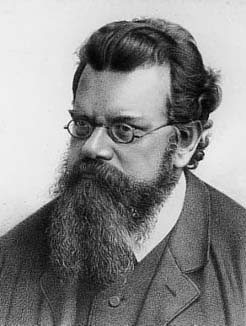
\includegraphics[scale=0.5]{Boltzmann}  
     \end{center}
    \end{minipage}&
    \begin{minipage}{0.45\textwidth} 
\tableofcontents[part=1]
 \end{minipage}
\end{tabular}
}
\section{Introdução}
\frame{\frametitle{Distribuições de Probabilidade}
  \begin{itemize}
  \item Mecânica Estatística determina a distribuição de energia 
em função dos níveis de energia.
\item Aplicações:
  \begin{itemize}
  \item Equilíbrio Químico
  \item Número de ligantes presos a uma molécula de DNA
  \item Problema dos Polímeros
  \end{itemize}
  \end{itemize}

}
\frame{\frametitle{Distribuições de Probabilidade}
  \begin{itemize}
  \item Níveis de Energia
  \item Estado Fundamental (``Ground State'')
  \item Níveis de energia do sistema $E_1,E_2,\ldots $
  \item Níveis de energia das partículas isoladas $\epsilon_1, \epsilon_2, \ldots $
  \end{itemize}
}


\section{Distribuição de Equilíbrio}

\frame{\frametitle{Entropia Boltzmann}
$$S=k\log W$$

onde
$$k=1.380662\times 10^{-25}J/K$$
e $W$ é a multiplicidade.

}

\frame{\frametitle{Justificativa para a definição de Boltzmann}
  Suponha que eu possua um sistema $S$ que pode ser dividido em duas
  partes iguais.$A$ e $B$ Se $A$ e $B$ interagem muito fracamente
então:

$$W=W_AW_B$$

$$\ln W=\ln W_A +\ln W_B$$

$$S=S_A+S_B$$

Esta propriedade é chamada de Extensividade. A Entropia oriunda historicamente 
da Termodinâmica satisfaz essa propriedade.
} 



\frame{\frametitle{Perspectiva
    Probabilística}

  Informação:

$$-\log p_i$$

Entropia:

$$\frac{S}{k}=-\sum_{j=1}^t p_j \ln p_j$$

Interpretação: a Entropia é o valor esperado da quantidade de
informação que eu recebo ao ser comunicado do resultado de um evento
aleatório.

}

\frame{\frametitle{Lançamento de dados}

  Considere um dado com $r$ lados.

  A multiplicidade de $N$ lançamentos nesse caso é:

$$W=\frac{N!}{n_1! \ldots n_r!}$$

A variável de interesse nesse caso é a freq. de ocorrência de cada um
dos lados.

$$p_r=\frac{n_r}{N}$$

$$\log W=N\log N-N- \sum_i (n_i\log n_i-n_i)=N\log N -\sum_i n_i\log n_i$$
}

\frame{\frametitle{Lançamento de dados}
$$\log W=\sum_i n_i \log N-n_i\log n_i=\sum_i -n_i\log \frac{n_i}{N}=
N\sum_i p_i\log p_i$$

$$ S=-N k\sum_i p_i \log p_i$$
}


\frame{\frametitle{Entropia sem vínculos}
$$\frac{S}{k}=-\sum_{j=1}^t p_j \ln p_j$$

$$\sum_i p_i=1$$

Usamos a técnica de multiplicadores de Lagrange:

$$\sum_i^t p_i \log p_i-\alpha \sum _i p_i$$


$$p_i=\frac{1}{t}$$
}


\frame{\frametitle{Questões Filosóficas}
  \begin{itemize}
  \item Qual é a origem probabilística da Entropia?
  \item Compatibilidade entre a Termodinâmica e a Mecânica Estatística.
  \item Qual é a relação entre Entropia e Informação?
  \item O que é de fato o Calor?
  \end{itemize}

}
\frame{\frametitle{Distribuição de Boltzmann}

$$\frac{S}{k}=-\sum_{j=1}^t p_j \ln p_j$$


$$dS=-k\sum_{j=1}^t(1+\ln p_j)dp_j$$

$$U=\langle E \rangle=\sum_{j=1}^t p_jE_j$$


}

\frame{\frametitle{Distribuição de Boltzmann}

  Agora devemos maximizar $S$ sujeita aos vínculos:

$$\sum_{j=1}^t p_j =1$$

$$\sum_{j=1}^t E_jp_j =U$$

} \frame{\frametitle{Distribuição de Boltzmann} Mostre que:

$$p_j=\frac{e^{-\beta E_j}}{Q}$$

$$Q=\sum_{j=1}^M e^{-\beta E_j}$$

$$\frac{p_i}{p_j}=e^{-(E_i-E_j)/kT}$$
}

\frame{\frametitle{Quem é beta?}

  Note que:

$$Z=\frac{S}{k}-\alpha -\beta U$$

$$-k T (Z+\alpha)=k T \beta U -TS$$

O que nos permite identificar:

$$F=U-TS$$

$$\beta=\frac{1}{k T}$$

}

\frame{\frametitle{Pressão Barométrica da Atmosfera}

  A energia de uma partícula a uma altura $z$ é:
$$\epsilon(z)=mgz$$

A razão do número de partículas é:

$$\frac{N(z)}{N(0)}=e^{-mgz/kT}$$

Se a temperatura for constante e o ar se comportar como gás ideal
temos que:

$$\frac{p(z)}{p(0)}=\frac{N(z)kT/V}{N(0)kT/V}=e^{-mgz/kT}$$

} \frame{\frametitle{Pressão Barométrica da Atmosfera}
  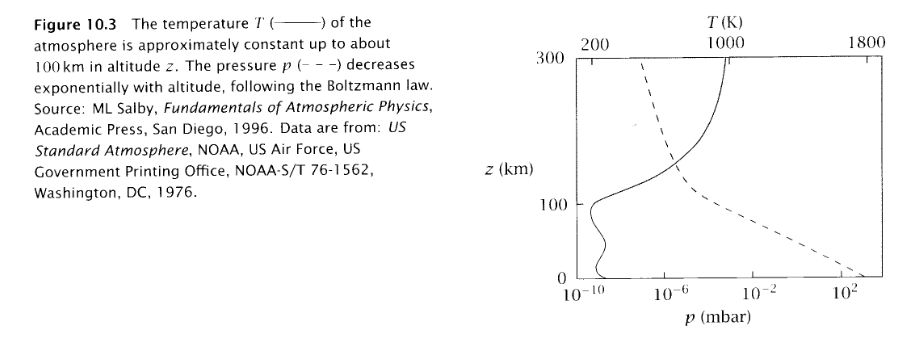
\includegraphics[scale=0.3]{pxz}

}


\frame{\frametitle{Distribuição de Velocidades} A energia de uma
  molécula de gás é:

$$\epsilon(v)=\frac{1}{2}mv^2$$


$$p(v_x)=\frac{e^{-\epsilon(v_x)/kT}}{\int_{-\infty}^{\infty}dxe^{-\epsilon(v_x)/kT}} 
=\frac{e^{-mv_x^2/kT}}{\int_{-\infty}^{\infty}dxe^{-mv_x^2/kT}}$$

$$p(v_x)        =\left(\frac{m}{2\pi k T}\right)^{1/2}e^{-mv_x^2/2 kT}$$ 

}

\frame{\frametitle{Distribuição de Velocidades}
$$\langle v_x^2 \rangle=\int_{-\infty}^{\infty}dx p(v_x)v_x^2
= \left(\frac{m}{2\pi k T}\right)^{1/2} \int_{-\infty}^{\infty}dx
e^{-mv_x^2/2 kT} v_x^2$$

$$\langle v_x^2 \rangle=\frac{kT}{m}$$

$$\frac{1}{2}m\langle v_x^2\rangle =\frac{1}{2}k T$$
}

\frame{\frametitle{Distribuição de Velocidades 3D}
$$\langle v^2 \rangle=\langle v_x^2+v_y^2+v_z^2 \rangle$$

$$\langle v^2 \rangle=\frac{3}{2}kT$$

$$p(v)=p(v_x)p(v_y)p(v_z)=\left(\frac{m}{2\pi k T}\right)^{3/2}e^{-mv^2/2 kT}$$
}


 \section{Função Partição}

\frame{\frametitle{Significado Físico}
A função de partição $Q$ mede o número de estados efetivamente acessíveis 
ao sistema.

$$Q=\sum_j^t e^{-E_j/kT}$$


Quando $T\rightarrow \infty$ $Q\rightarrow t$, quando $T\rightarrow 0$
o único estado ocupado é o fundamental e $p(E_1)=1$. 

}

\frame{\frametitle{Densidade de Estados}

$W(E)$ mede o número de estados microscópicos com energia $E$. 

No exemplo dos polímeros $W(\epsilon_o)=4$ e $W(0)=1$.  Neste caso

$$Q=1e^{-0/kT}+4e^{-\epsilon_o/k T}$$

A função de partição pode ser escrita nos casos de interesse como:

$$Q=\sum_{l=1}^{l_{max}}W(E_l)e^{-E_l/k T}$$

Em um sistema, os estados com probabilidade de ocupação razoável satisfazem 
$E\sim kT$, pois se $E>kT$ seu peso de Boltzmann é muito pequeno,
$E<k T$ sua multiplicidade $W$ é muito pequena. 
}

 \frame{\frametitle{Distribuição de Boltzmann}
 \begin{tabular}{c c}
     \begin{minipage}{0.45\textwidth}
       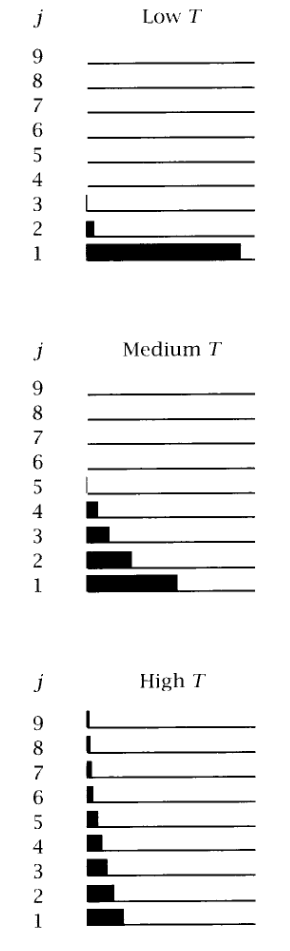
\includegraphics[scale=0.2]{boltz}
     \end{minipage}&

     \begin{minipage}{0.45\textwidth}
       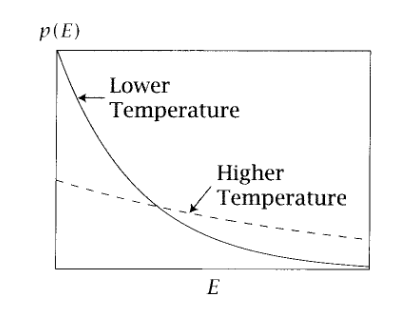
\includegraphics[scale=0.4]{boltz3}
     \end{minipage}
   \end{tabular}
 }


 \frame{\frametitle{Colapso Polimérico}
 \begin{tabular}{c c}
     \begin{minipage}{0.45\textwidth}
 $$F_{C}=U_{dimero}-TS_{dimero}$$
 $$F_{C}=-\epsilon$$
 $$F_{O}=-kT\ln 4$$

     \end{minipage}&
     \begin{minipage}{0.45\textwidth}
       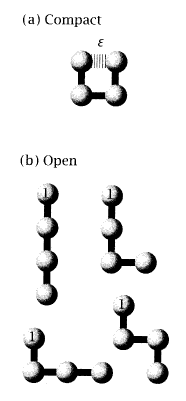
\includegraphics[scale=0.4]{colapsopolimero}
     \end{minipage}
   \end{tabular}
 }

\frame{\frametitle{Colapso Polimérico}
$$Q=1e^{-0/kT}+4e^{-\epsilon_o/k T}=1+4e^{-\epsilon_o/k T}$$

$$p_C=\frac{1}{1+4e^{-\epsilon_o/k T}}$$

$$p_O=\frac{4 e^{-\epsilon_o/k T}}{1+4e^{-\epsilon_o/k T}}$$

\begin{center}
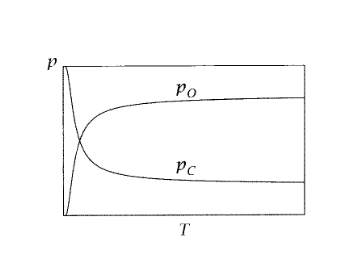
\includegraphics[scale=0.3]{Qcolapso}  
\end{center}
}


\frame{\frametitle{Função Partição Partículas Independentes}

Considere o caso em que temos $N$ partículas independentes
e distinguíveis (ex. cristal):

$$Q=\prod_{a=1}^N\sum_{j=1}^t e^{-\epsilon_j^a}$$
$$Q=\left( \sum_{j=1}^t e^{-\epsilon_j} \right)^N=q^N$$
$$q=\sum_{j=1}^t e^{-\epsilon_j}$$

}

\frame{\frametitle{Função Partição Partículas Independentes}

Considere o caso em que temos $N$ partículas independentes
e indistinguíveis (ex. gás):

$$Q=\frac{q^N}{N!}$$
$$q=\sum_{j=1}^t e^{-\epsilon_j}$$

}

 \section{Propriedades Termodinâmicas}


\frame{\frametitle{Energia Interna}

Todas propriedades termodinâmicas podem ser obtidas 
se conhecemos a função partição $Q$

$$U=\sum_{j=1}^t p_jE_j=\frac{1}{Q}\sum_{j=1}^t E_je^{-\beta E_j}$$

$$\left( \frac{\partial Q}{\partial \beta} \right)=
-\sum_{j=1}^t E_j e^{-\beta E_j}$$

$$U=-\frac{1}{Q}\left( \frac{\partial Q}{\partial \beta} \right)=
-\left( \frac{\partial \ln Q}{\partial \beta} \right)$$

Como $\beta =1/k T$ temos:
$$\left( \frac{\partial \beta}{\partial T} \right)=-\frac{1}{kT^2}$$

}

\frame{\frametitle{Energia Interna}
Finalmente


$$U=k T^2\left( \frac{\partial \ln Q}{\partial \beta} \right)$$

}

\frame{\frametitle{Entropia}

$$\frac{S}{k}=-\sum_{j=1}^t -p_j\ln p_j$$

$$\frac{S}{k}=-\sum_{j=1}^t\frac{e^{-\beta E_j}}{Q}
\left(-\ln Q -\frac{E_j}{k T}\right)$$

$$S=k\ln Q+\frac{U}{T}=
k\ln Q+k T \left( \frac{\partial \ln Q}{\partial \beta} \right)$$
}


\frame{\frametitle{Entropia}
 
 $$U=k T^2\left( \frac{\partial \ln Q}{\partial \beta} \right) $$

 $$ S=k\ln Q+k T \left( \frac{\partial \ln Q}{\partial \beta} \right)$$

 $$F=U-TS=-k T\ln Q$$

 $$\mu=\left( \frac{\partial F}{\partial N} \right)_{T,N}
      =-kT\left( \frac{\partial \ln Q}{\partial N} \right)$$

 $$p=\left( \frac{\partial F}{\partial V} \right)_{T,N}
     =-kT\left( \frac{\partial \ln Q}{\partial V} \right)$$
}

\frame{\frametitle{Sistemas com dois estados}

Neste sistema temos $N$ partículas com níveis de energia $\epsilon=0$
e $\epsilon_o$. Este modelo pode ser aplicado em muitas 
situações de interesse físico:
\begin{itemize}
\item spins em um campo magnético
\item partículas excitadas pela radiação
\item os polímeros descritos anteriormente
\end{itemize}

}

\frame{\frametitle{Sistemas com dois estados}
$$q=1+e^{-\beta \epsilon_o}$$
$$p_1=\frac{1}{q}\quad p_2=\frac{e^{-\beta \epsilon_o}}{q}$$
$$\langle \epsilon \rangle = -\frac{1}{q}\left( 
\frac{\partial q}{\partial \beta}\right)=\frac{\epsilon_o e^{-\beta \epsilon_o}}{1+e^{-\beta\epsilon_o}}=\frac{\epsilon_o e^{-\epsilon_o/k T}}{1+e^{-\epsilon_o/kT}}
$$
\begin{center}
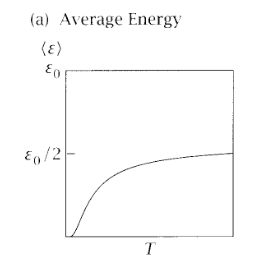
\includegraphics[scale=0.3]{ExT}  
\end{center}
}


\frame{\frametitle{Sistemas com dois estados}
$$C_V=  N\left( \frac{\partial \langle \epsilon \rangle}{\partial T} \right)=
N\left( \frac{\partial \langle \epsilon \rangle}{\partial \beta} \right)\left( \frac{\partial \beta }{\partial T} \right)
$$

$$C_V=\frac{N\epsilon^2}{kT^ 2}\frac{e^{-\beta \epsilon_o}}{(1+e^{-\beta \epsilon_o})^2}$$

 \begin{center}
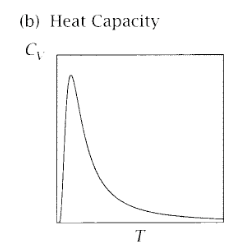
\includegraphics[scale=0.3]{CvxT}  
\end{center}
}
\frame{\frametitle{Sistemas com dois estados}
$$S=k\ln Q+k T \left( \frac{\partial \ln Q}{\partial \beta} \right)$$
$$\frac{S}{N}= \frac{\epsilon_oe^{-\beta \epsilon_o}}{T(1+e^{-\beta\epsilon_o})} +k\ln (1+e^{-\beta \epsilon_o}) $$

$$F=-N\ln q=-\ln (1+e^{-\beta\epsilon_o})$$
}

\frame{\frametitle{Lei de Curie}
Considere um spin com momento magnético $\mu_o$ sob a ação de um campo 
magnético $B$, os dois níveis de energia são:
$$\epsilon_1=-\mu_o B\quad \mbox{e}\quad \epsilon_2=\mu_oB$$ 
Reescalando a energia para que $\epsilon_1=0$, $\epsilon_2=2 \mu_o B$
$$q=1+e^{-2\mu_o B/KT}$$

}

\frame{\frametitle{Lei de Curie}
$$p_1=\frac{1}{q}\quad p_2=\frac{e^{-2\mu_o B/kT}}{q}$$
$$\langle \mu \rangle =\mu_op_1-\mu_op_2=\mu_o\frac{1-e^{-2\mu_oB/kT}}{1+e^{-2\mu_oB/kT}}$$

$$\langle \mu \rangle =\mu_o\tanh\left( \frac{\mu_o B}{k T}\right)$$
 \begin{center}
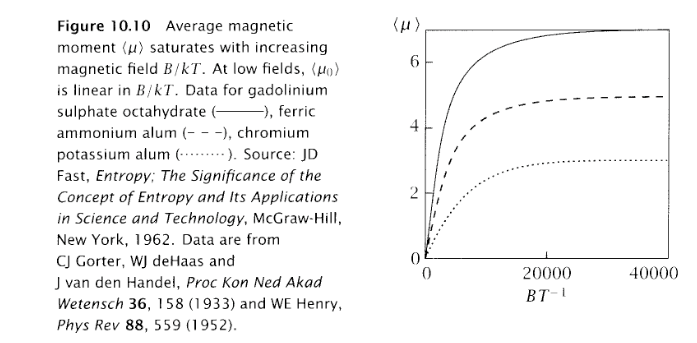
\includegraphics[scale=0.3]{curie}  
\end{center}

}

\section{Ensembles}


\frame{\frametitle{Ensembles}

Um ensemble é o conjunto de micro-estados compatíveis com 
os vínculos do sistema. Na Mecânica Estatística trabalhamos com 
3 Ensembles:
\begin{description}
\item[Micro-canônico] $E$, $V$ e $N$ constantes
\item[Canônico] $T$, $V$ e $N$ constante, E flutua
\item[Gran-canônico] $T$, $V$ e $\mu$ constante $E$ e $N$ flutuam
\end{description}
}


\frame{\frametitle{Micro-canônico}
Neste caso maximizamos $S$ sujeito a um único vínculo:
$$\sum p_i=1$$, neste caso podemos mostrar que $p_i=1/t$ e
$$S=k\ln W$$
}

\end{document}
